\documentclass[a4paper,10pt]{article}
\usepackage[utf8]{inputenc}
\usepackage{listings}
\usepackage{graphicx}
\usepackage{subcaption}
\usepackage{adjustbox}
\graphicspath{ {./images/} }
%opening
\title{Compte rendu TP2 : Programmation générique}
\date{10/11/20}
\author{Commandeur N. - Verdant B}

\begin{document}

\maketitle
\pagenumbering{gobble}
\newpage

  \pagenumbering{arabic}
  \section{Introduction}
  Pour compiler les sources, il suffit de faire un make. Chaque réponse fera l'affaire d'une section avec la commande correspondante.


  \section{Définition d'une classe pour représenter des images arbitraires}
  Utilisation de la classe générique Image2D pour représenter une image en niveau de gris :
  \begin{lstlisting}[language=Bash]
  $ ./testGrayLevelImage2D  
    5 5 5 5 5 5 5 5
    5 5 5 5 5 5 5 5
    5 5 5 5 5 5 5 5
    5 5 5 5 5 5 5 5
    5 5 5 5 5 5 5 5
    5 5 5 5 5 5 5 5
    5 5 5 5 5 5 5 5
    5 5 5 5 5 5 5 5
  \end{lstlisting}
  \section{Introduction des images couleurs}
  Utilisation de la classe générique Image2D pour représenter une image en couleur.
  \begin{lstlisting}[language=Bash]
  $ ./testColorImage2DBash
  255 0 255| 255 0 255| 255 0 255| 
  255 0 255| 255 0 255| 255 0 255| 
  255 0 255| 255 0 255| 255 0 255| 
  \end{lstlisting}
    \pagebreak
    \section{Premier itérateur sur images quelconques}
     Utilisation de la classe générique Image2D pour représenter une image en couleur,
  \begin{lstlisting}[language=Bash]
  $ ./testColorImage2D
  \end{lstlisting}
    \section{Un importeur / exporteur PBM générique}
    On va écrire une classe pour écrire et lire un fichier, en spécialisant pour la couleur et les nuances de gris. On va réutiliser la fonction permettant de créer l'image et l'écrire dans le fichier  \emph{colors.ppm}
    \begin{lstlisting}[language=Bash]
  $ ./testColorImage2D
  $ display colors.ppm
  \end{lstlisting}
  \begin{center}
    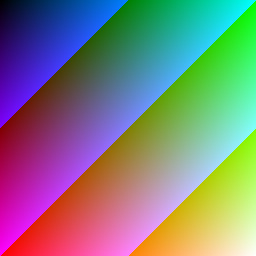
\includegraphics[scale=0.75]{colors}
    \end{center}
    \pagebreak
    \section{Premier test: on inverse les canaux rouge et bleu}
    Grâce à nos fonctions de lecture et écriture, on peut commencer à traiter les images. On va lire une image et écrire une nouvelle en changeant la couleur de chaque pixel en inversant le bleu et le rouge. Il faut donner une image en entrée et une image en sortie.
    \begin{lstlisting}[language=Bash]
  $ ./invert-blue-red patinoire.ppm patinoire-inv.ppm
  $ display patinoire-inv.ppm
  \end{lstlisting}
   \begin{figure}[h]
   \begin{subfigure}{0.6\textwidth}
    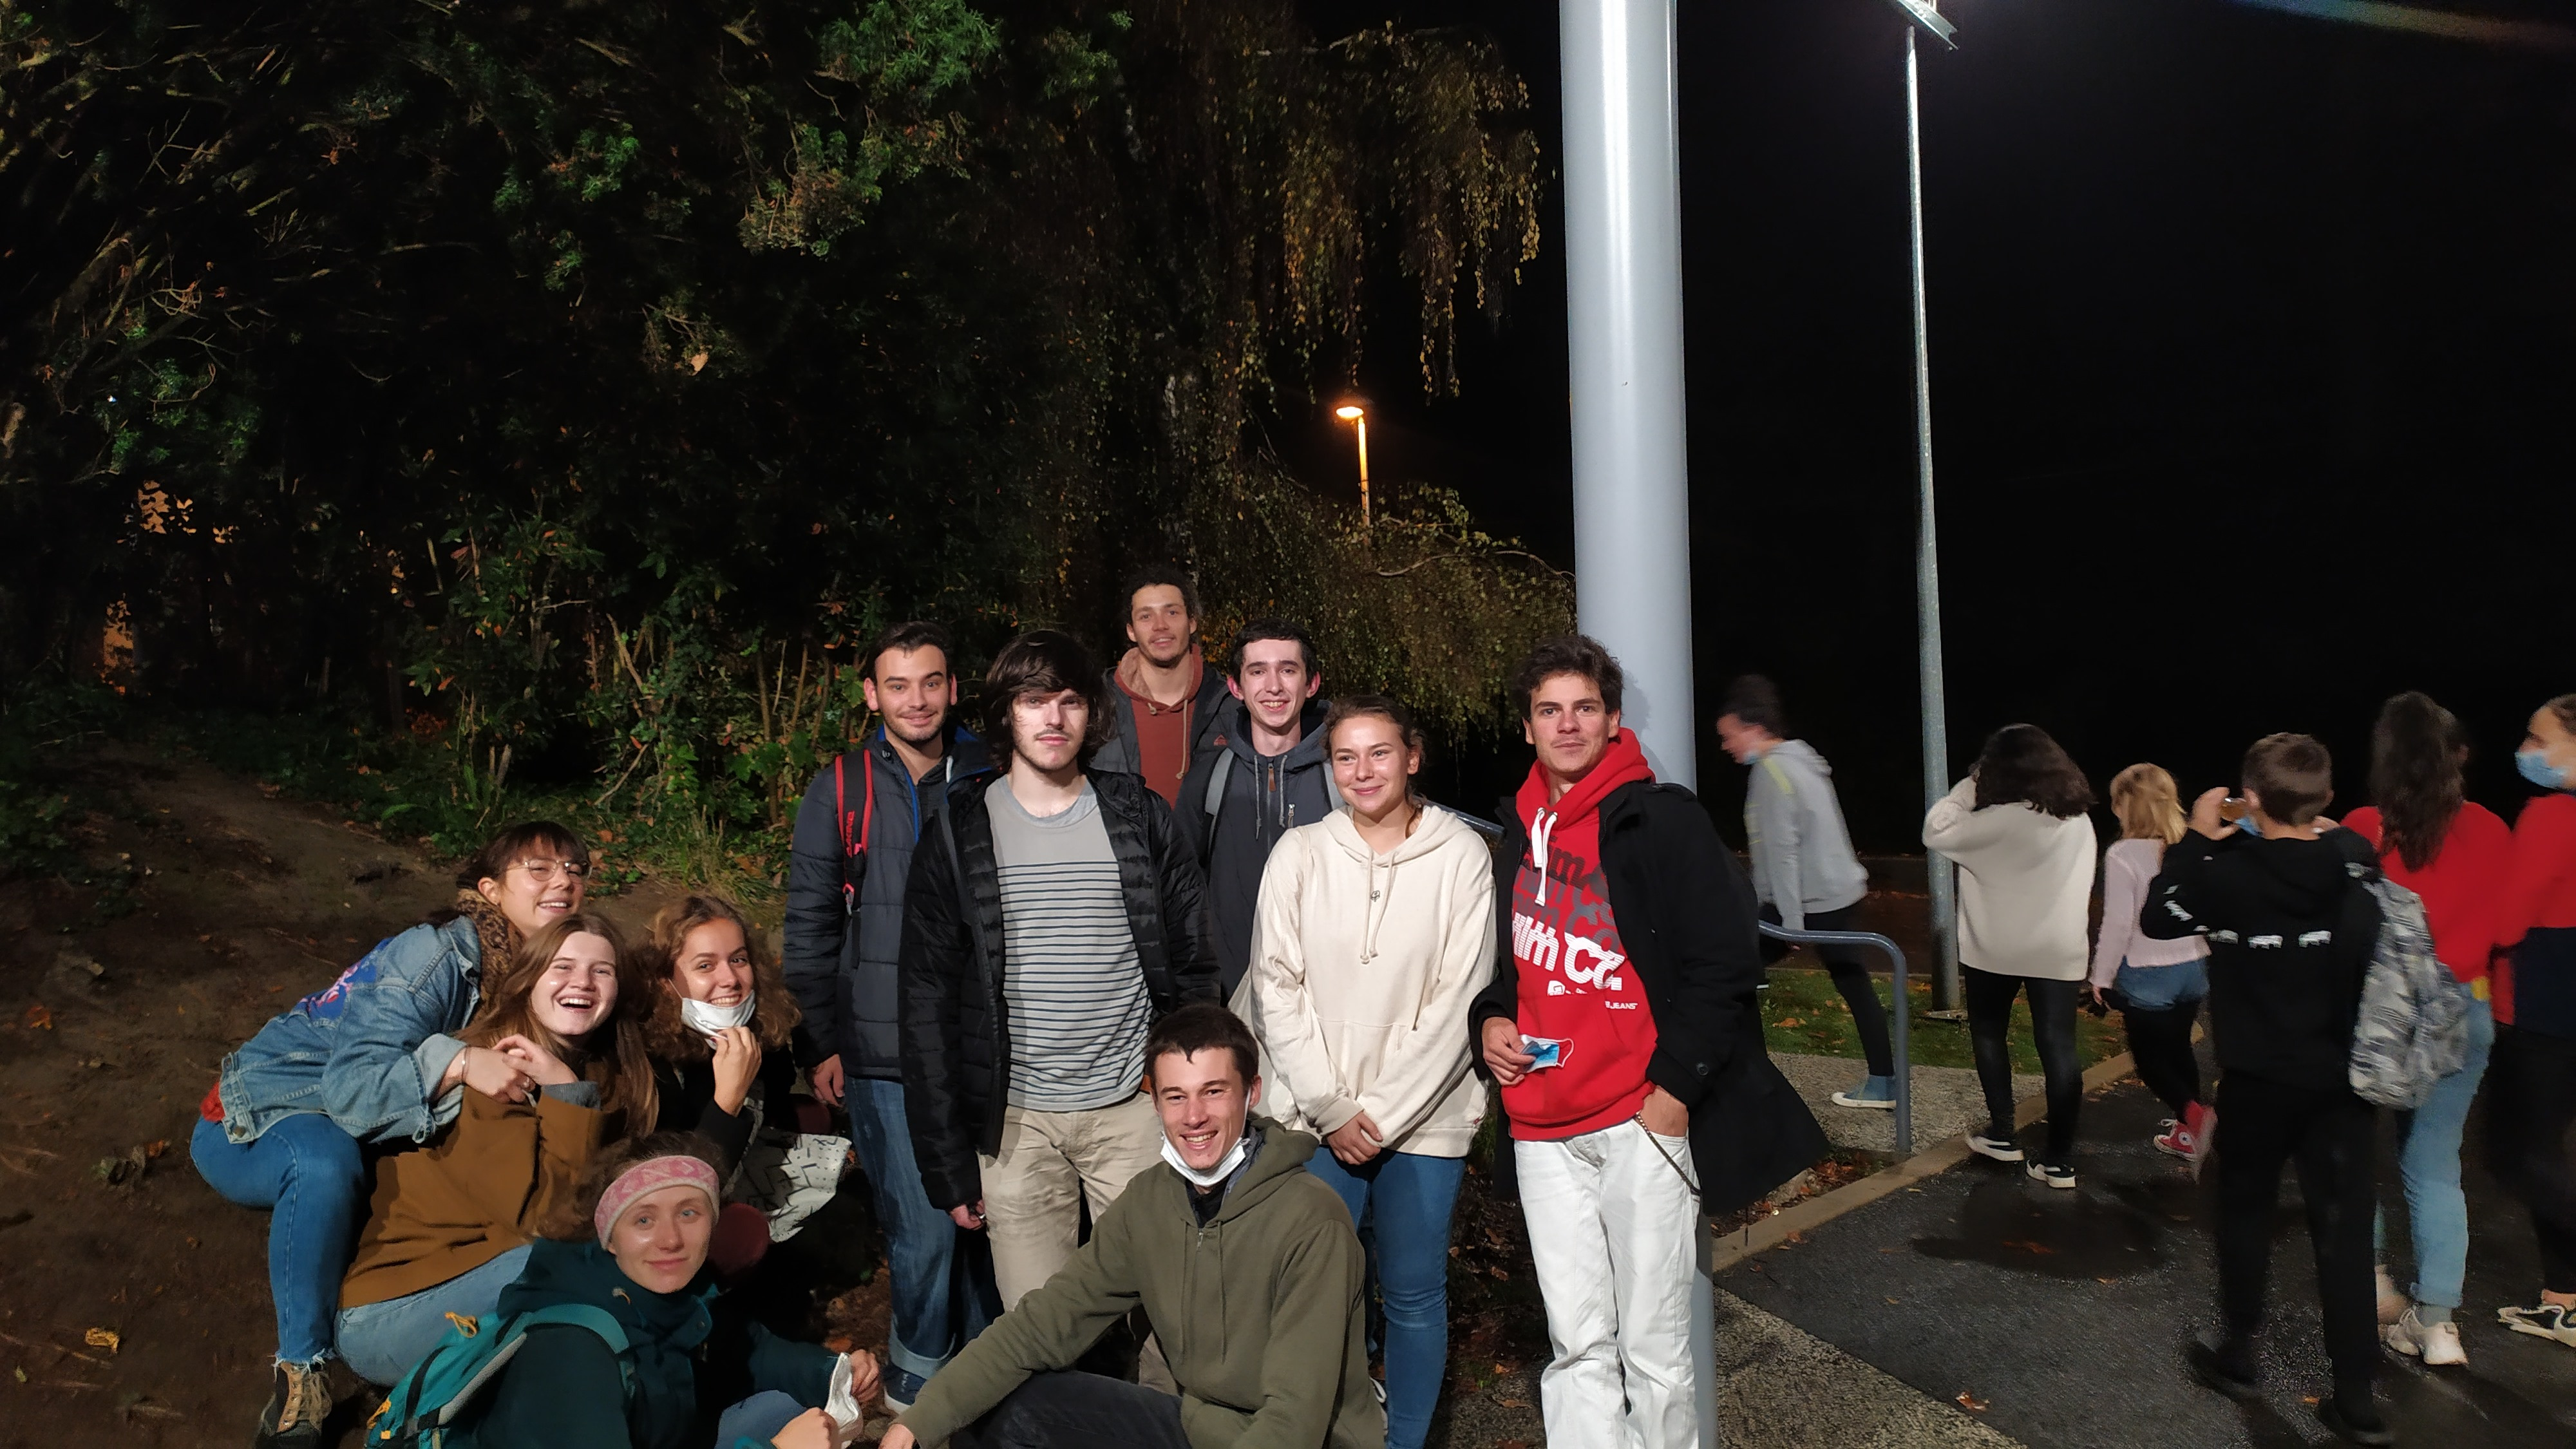
\includegraphics[width=1\linewidth, height=4cm]{patinoire}   
    \end{subfigure}
     \begin{subfigure}{0.6\textwidth}
    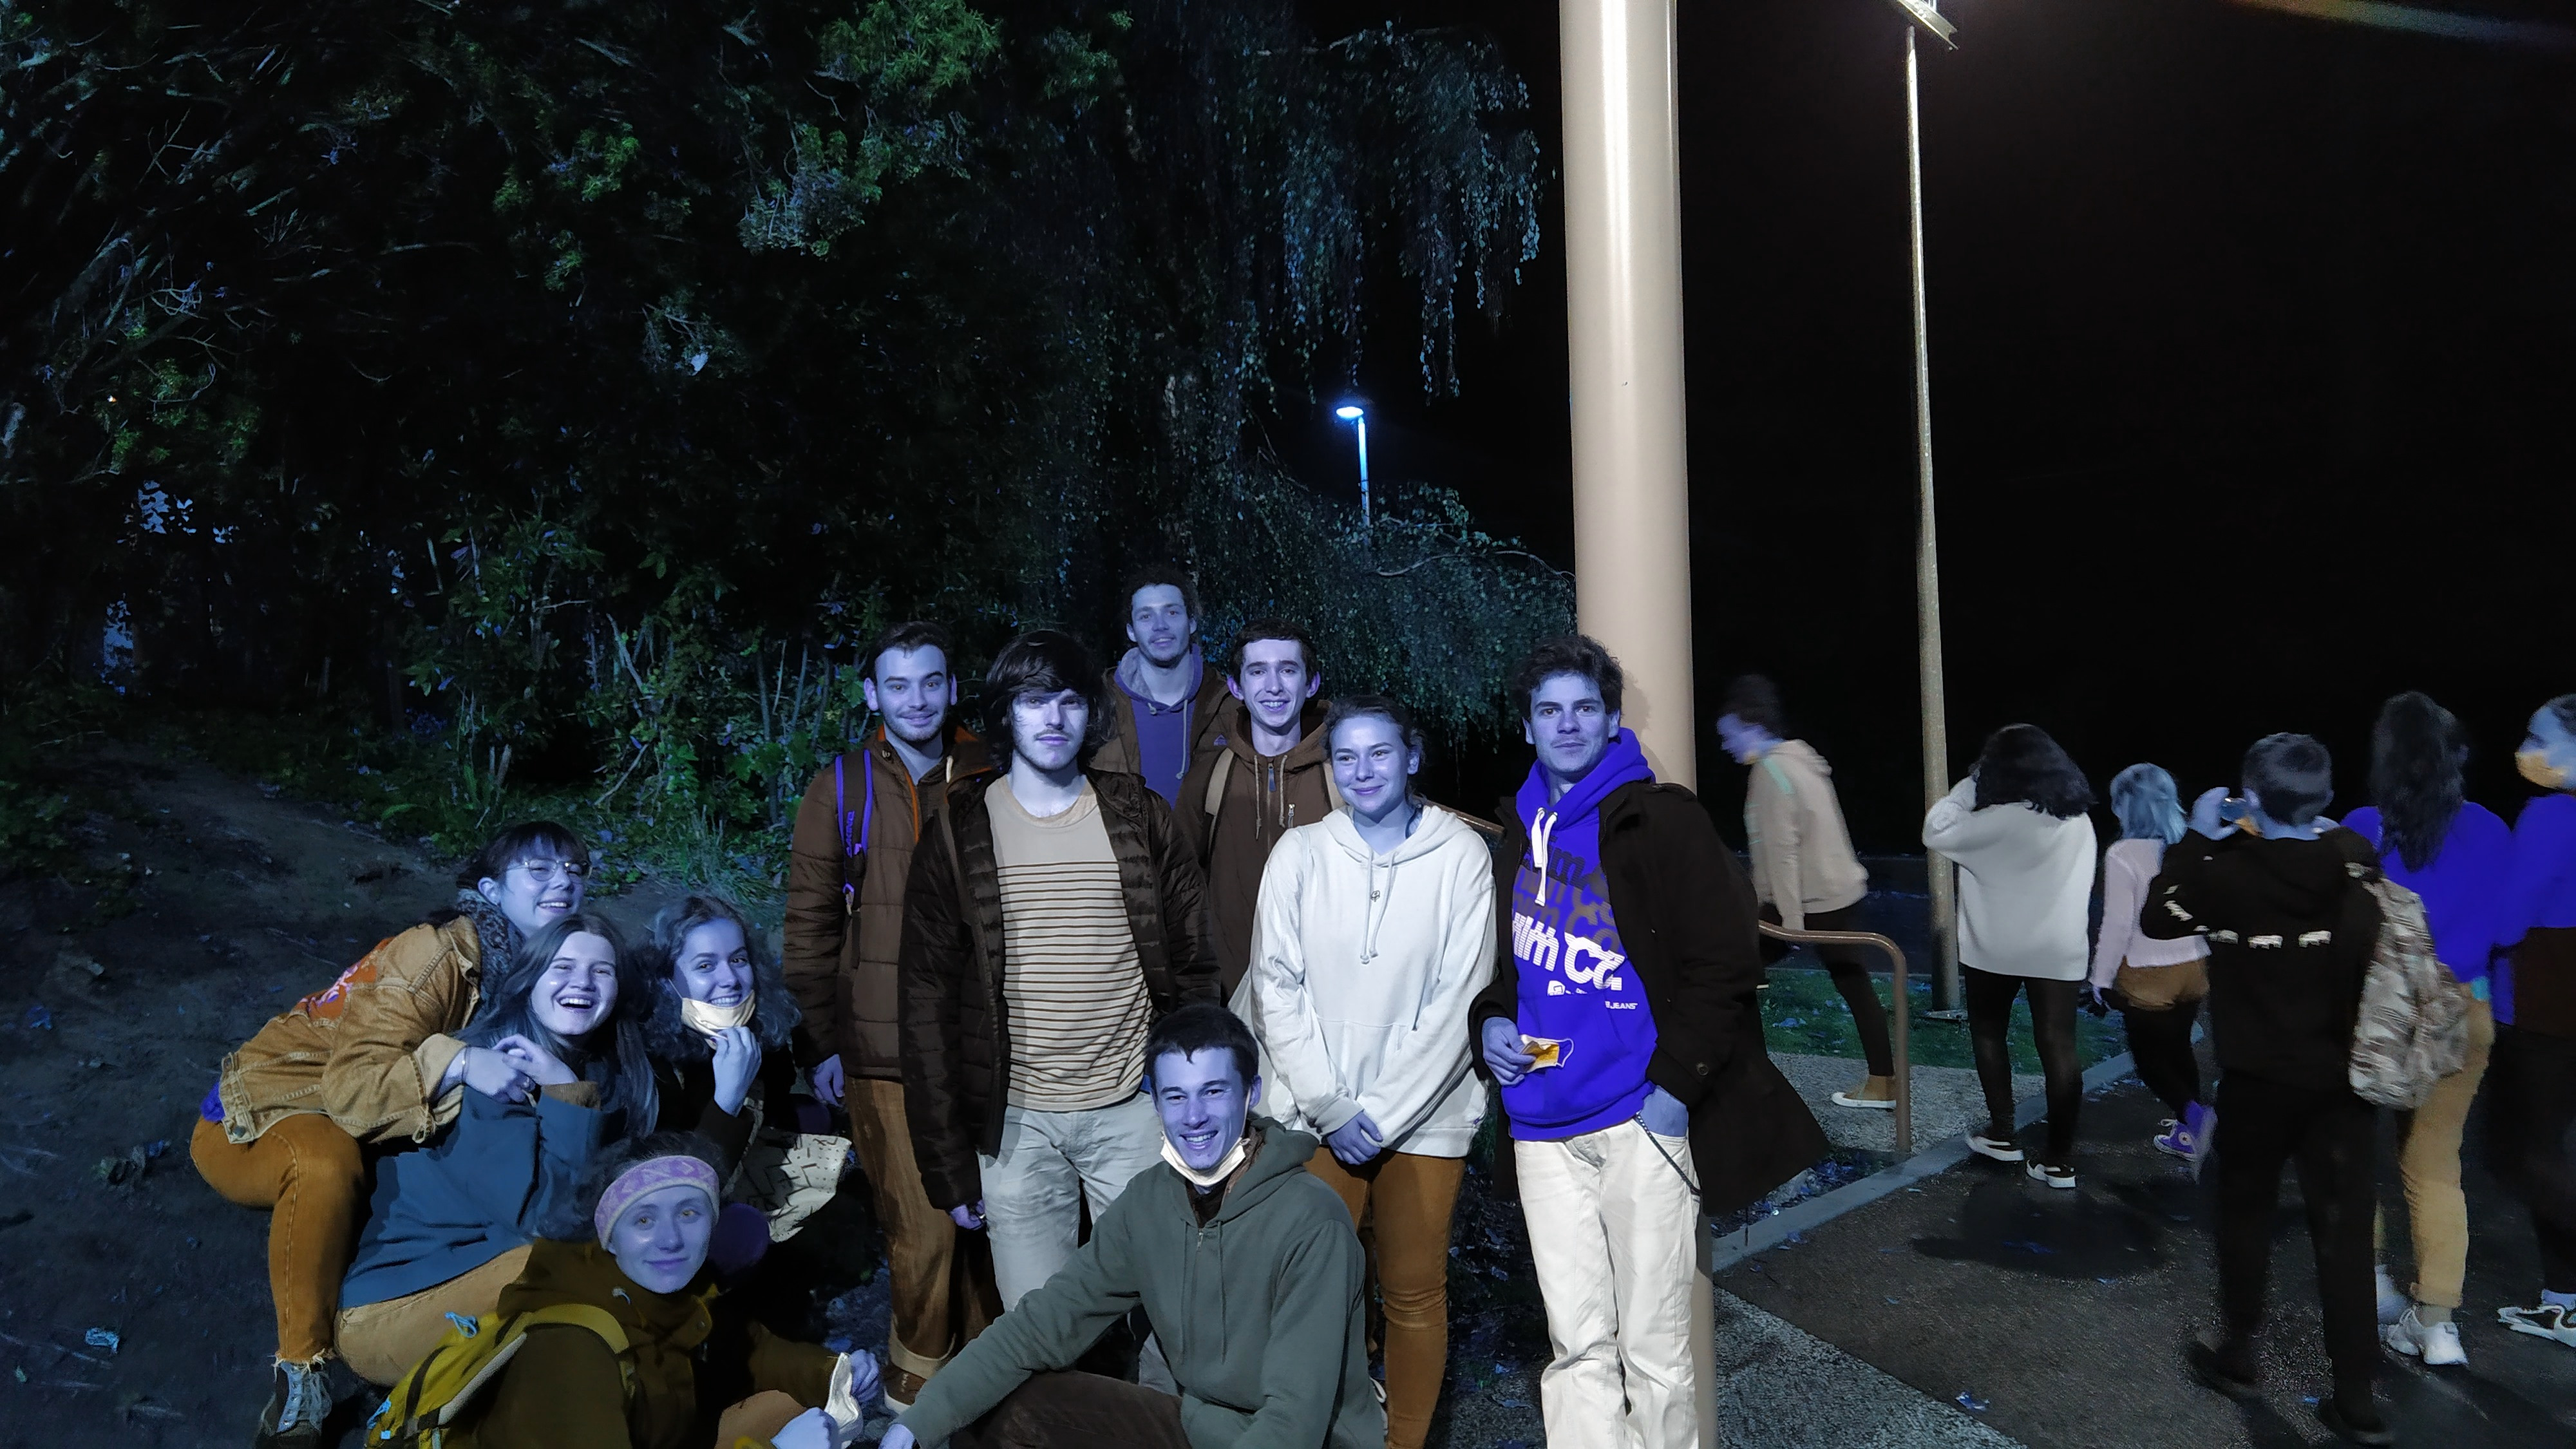
\includegraphics[width=1\linewidth, height=4cm]{patinoire-inv}   
    \end{subfigure}
    \end{figure}
    \pagebreak
    \section{On rajoute les accesseurs et un itérateur générique}
    On va définir des itérateurs sélectifs qui ne voient qu'une composante de la couleur (en lecture et en écriture). Plutôt que de les réécrire à chaque fois, on définit la notion d'accesseur, puis nos nouveaux itérateurs seront paramétrés par un accesseur. Grâce à nos nouveaux accesseur, on va pouvoir sauvegarder les 3 channels de couleurs sous forme de niveau de gris.
    \begin{lstlisting}[language=Bash]
  $ ./save-all-channel patinoire.ppm
  $ display patinoire_blue.pgm
  $ display patinoire_red.pgm
  $ display patinoire_green.pgm
  \end{lstlisting}
    \begin{figure}[h]
   \begin{subfigure}{0.6\textwidth}
    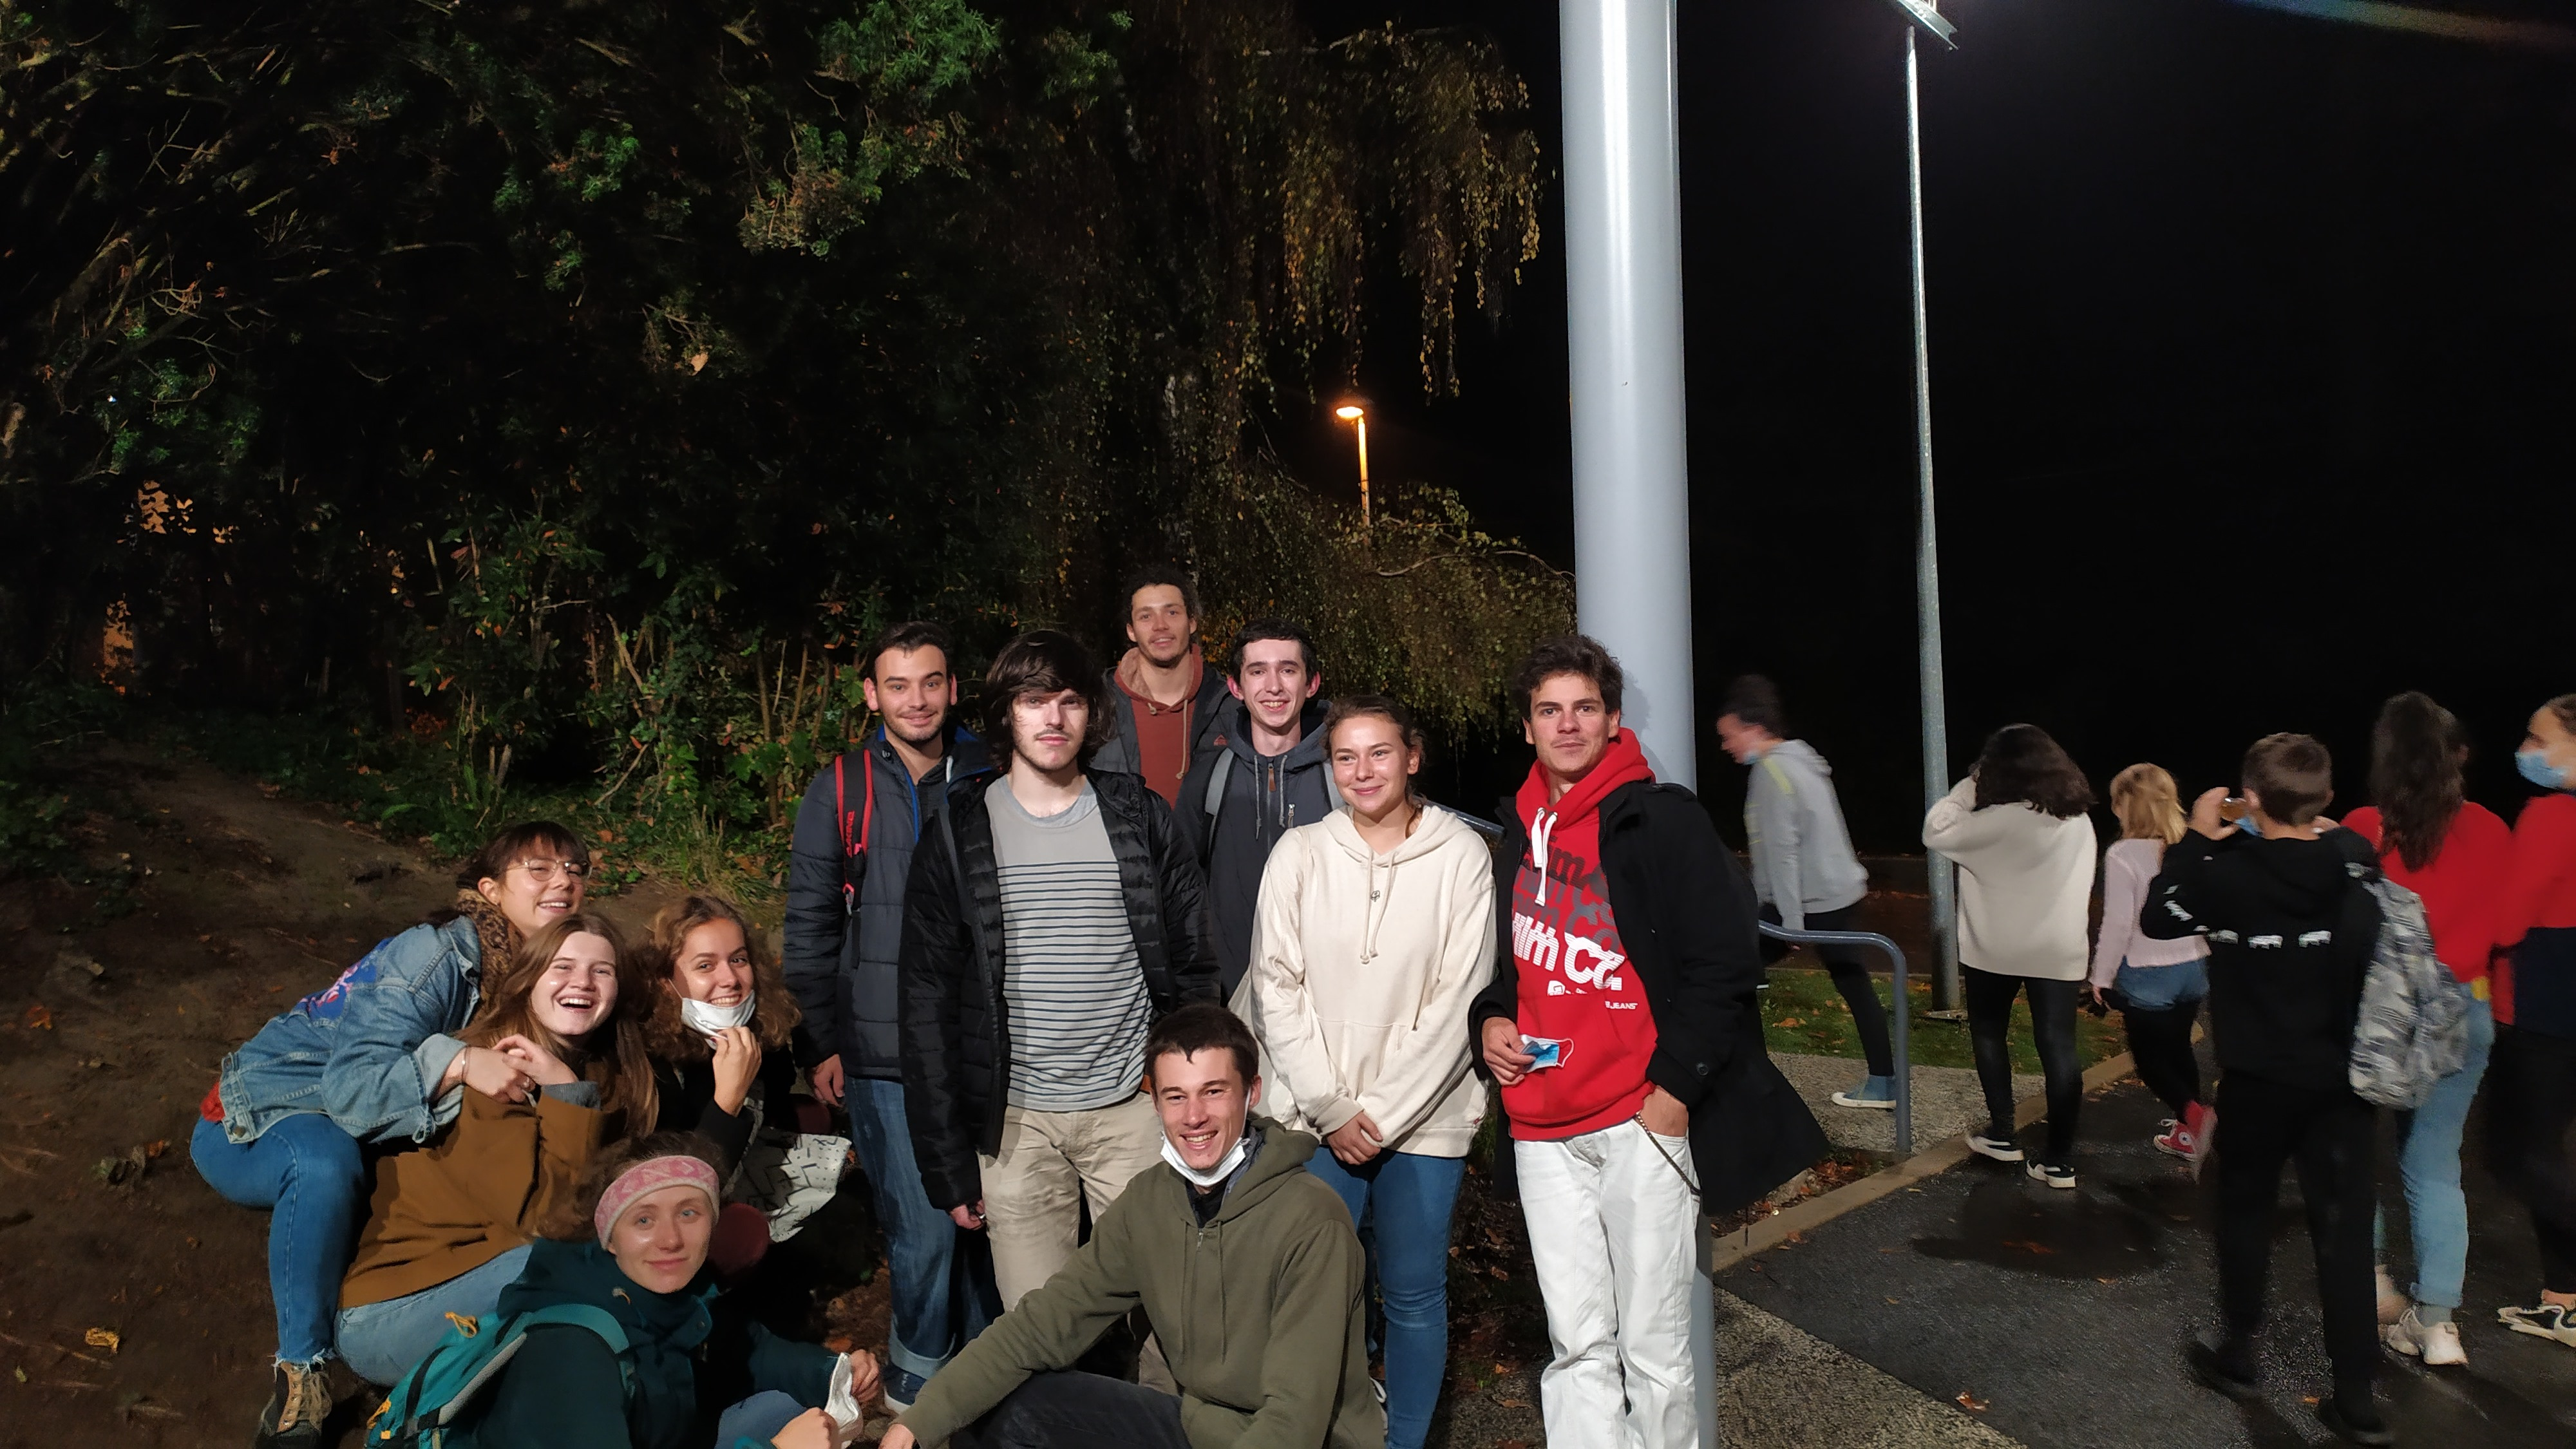
\includegraphics[width=1\linewidth, height=4cm]{patinoire}
    \caption{Image originale}
    \label{fig:patinoireOrigin}
    \end{subfigure}
     \begin{subfigure}{0.6\textwidth}
    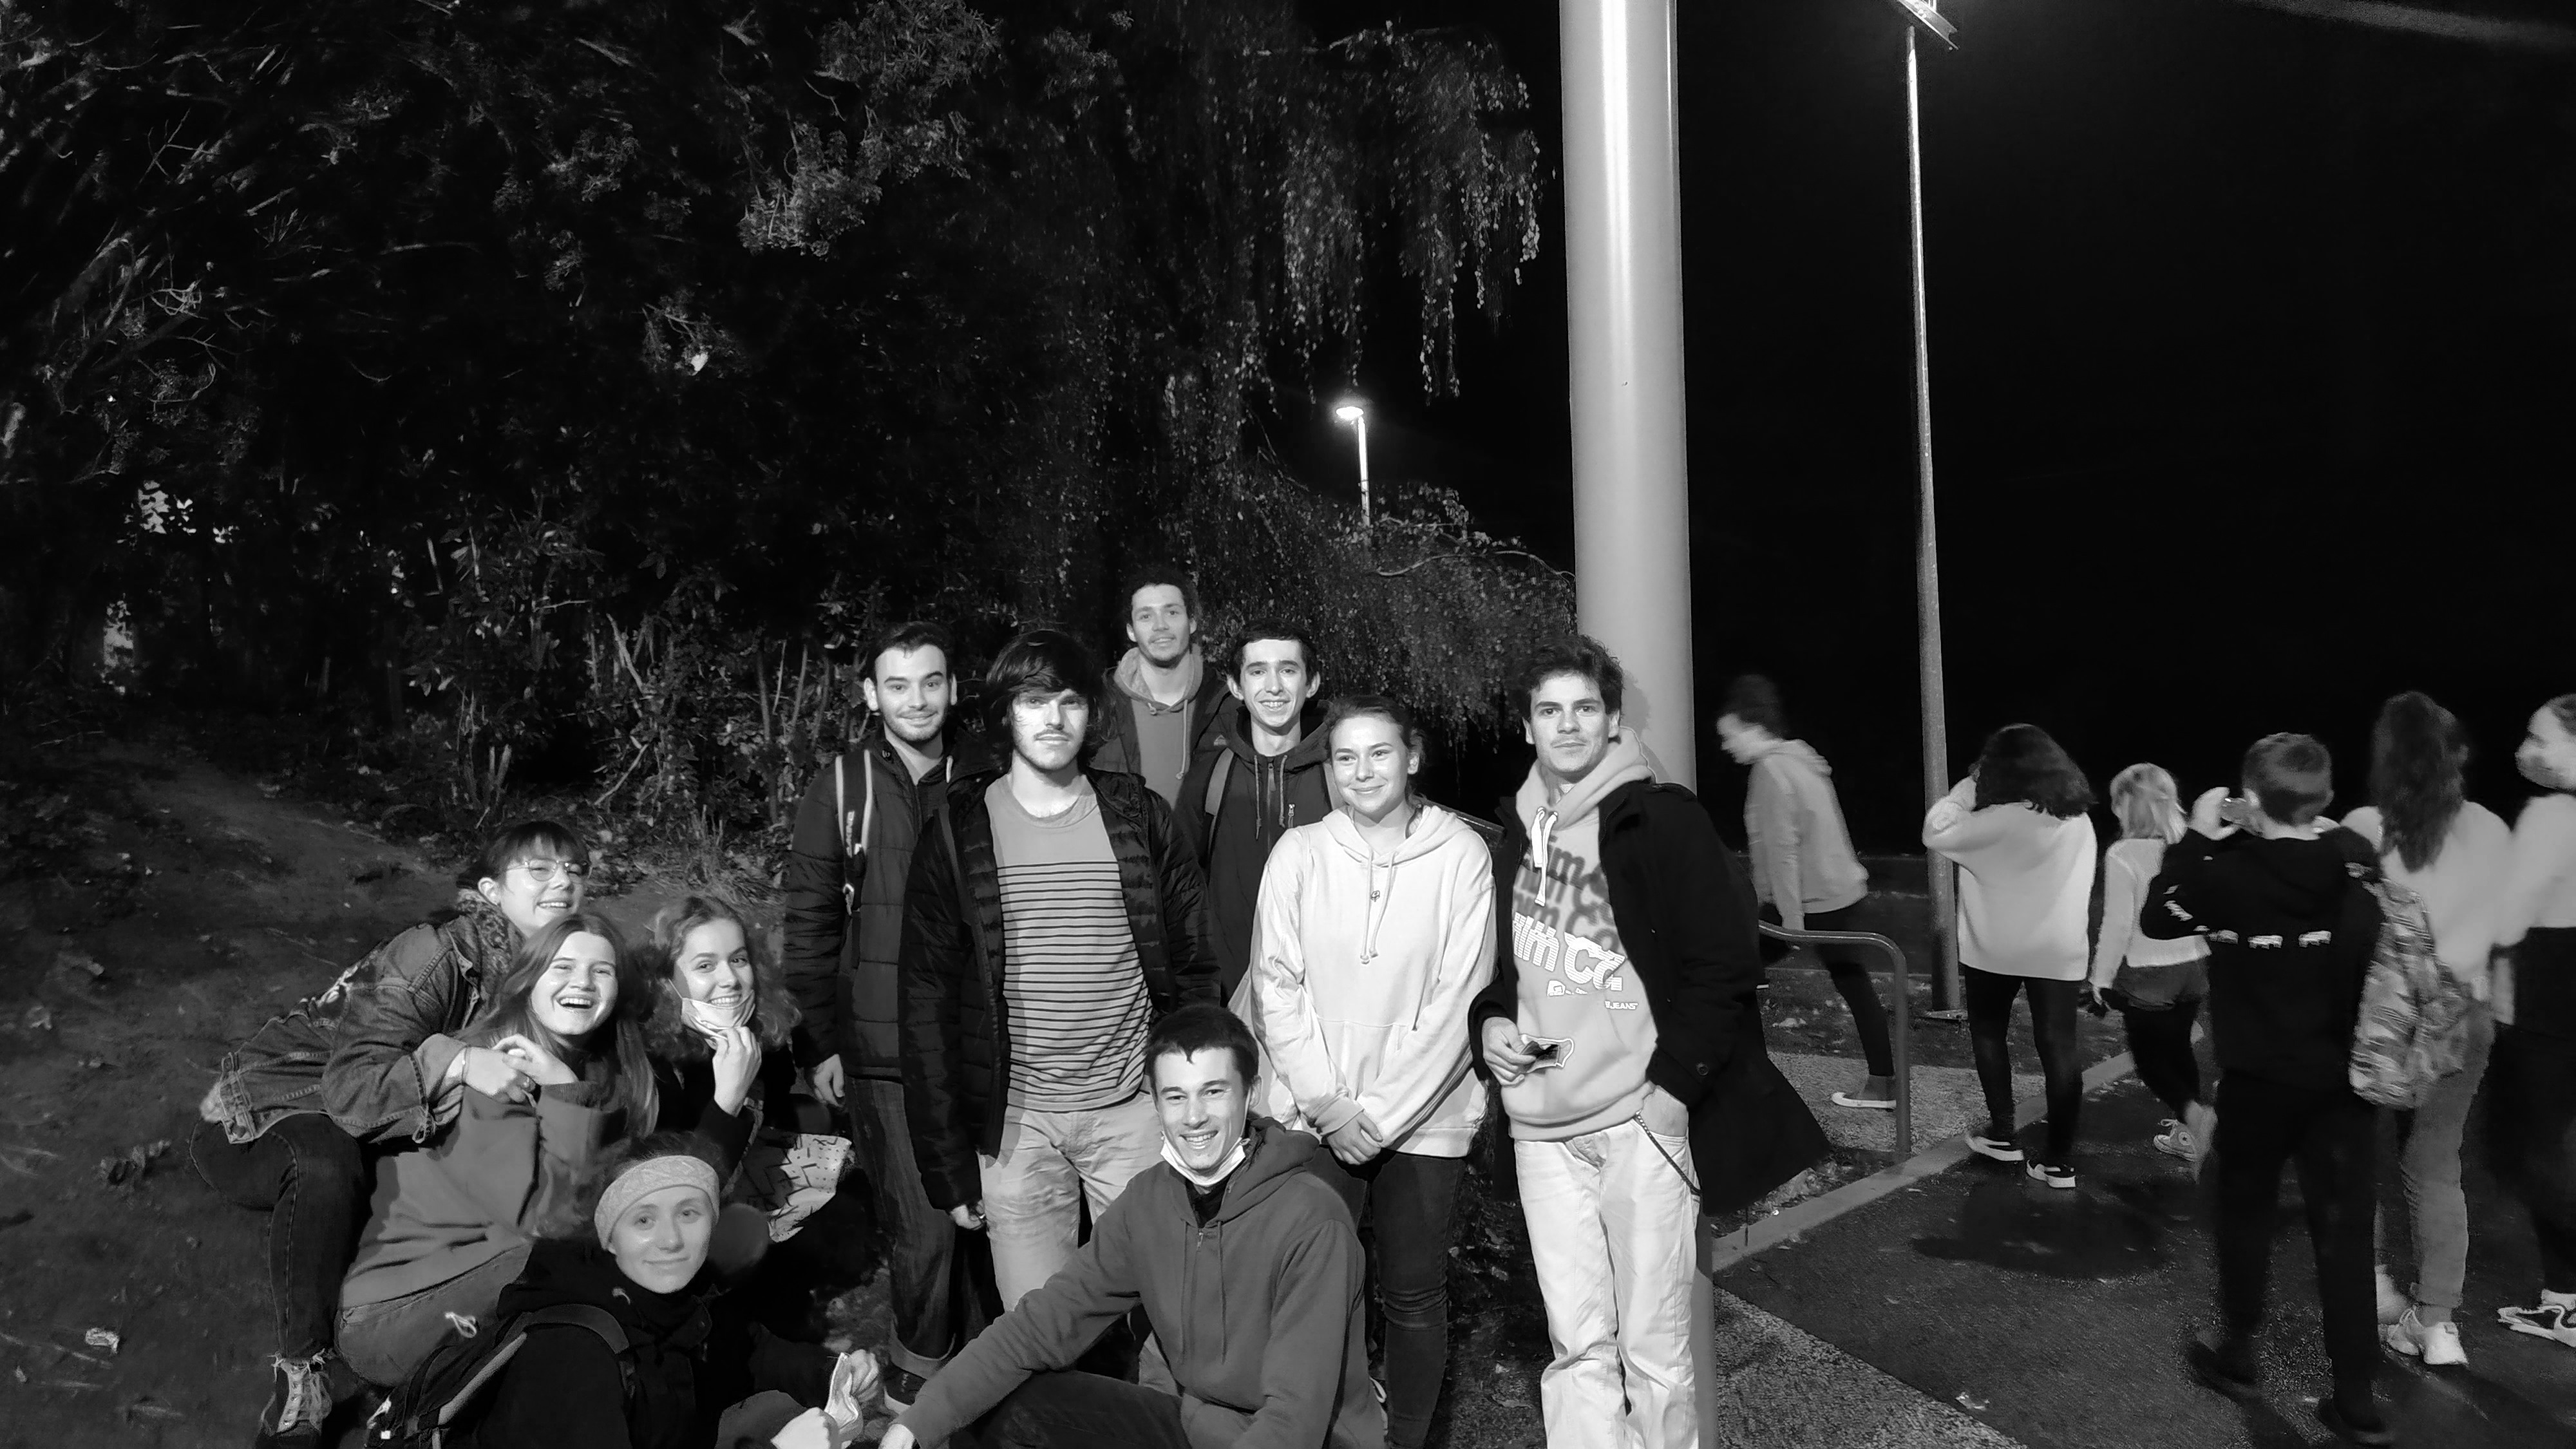
\includegraphics[width=1\linewidth, height=4cm]{patinoire_red}   
    \caption{Image des niveaux de gris du rouge}
    \label{fig:patinoireRed}
    \end{subfigure}
     \begin{subfigure}{0.6\textwidth}
    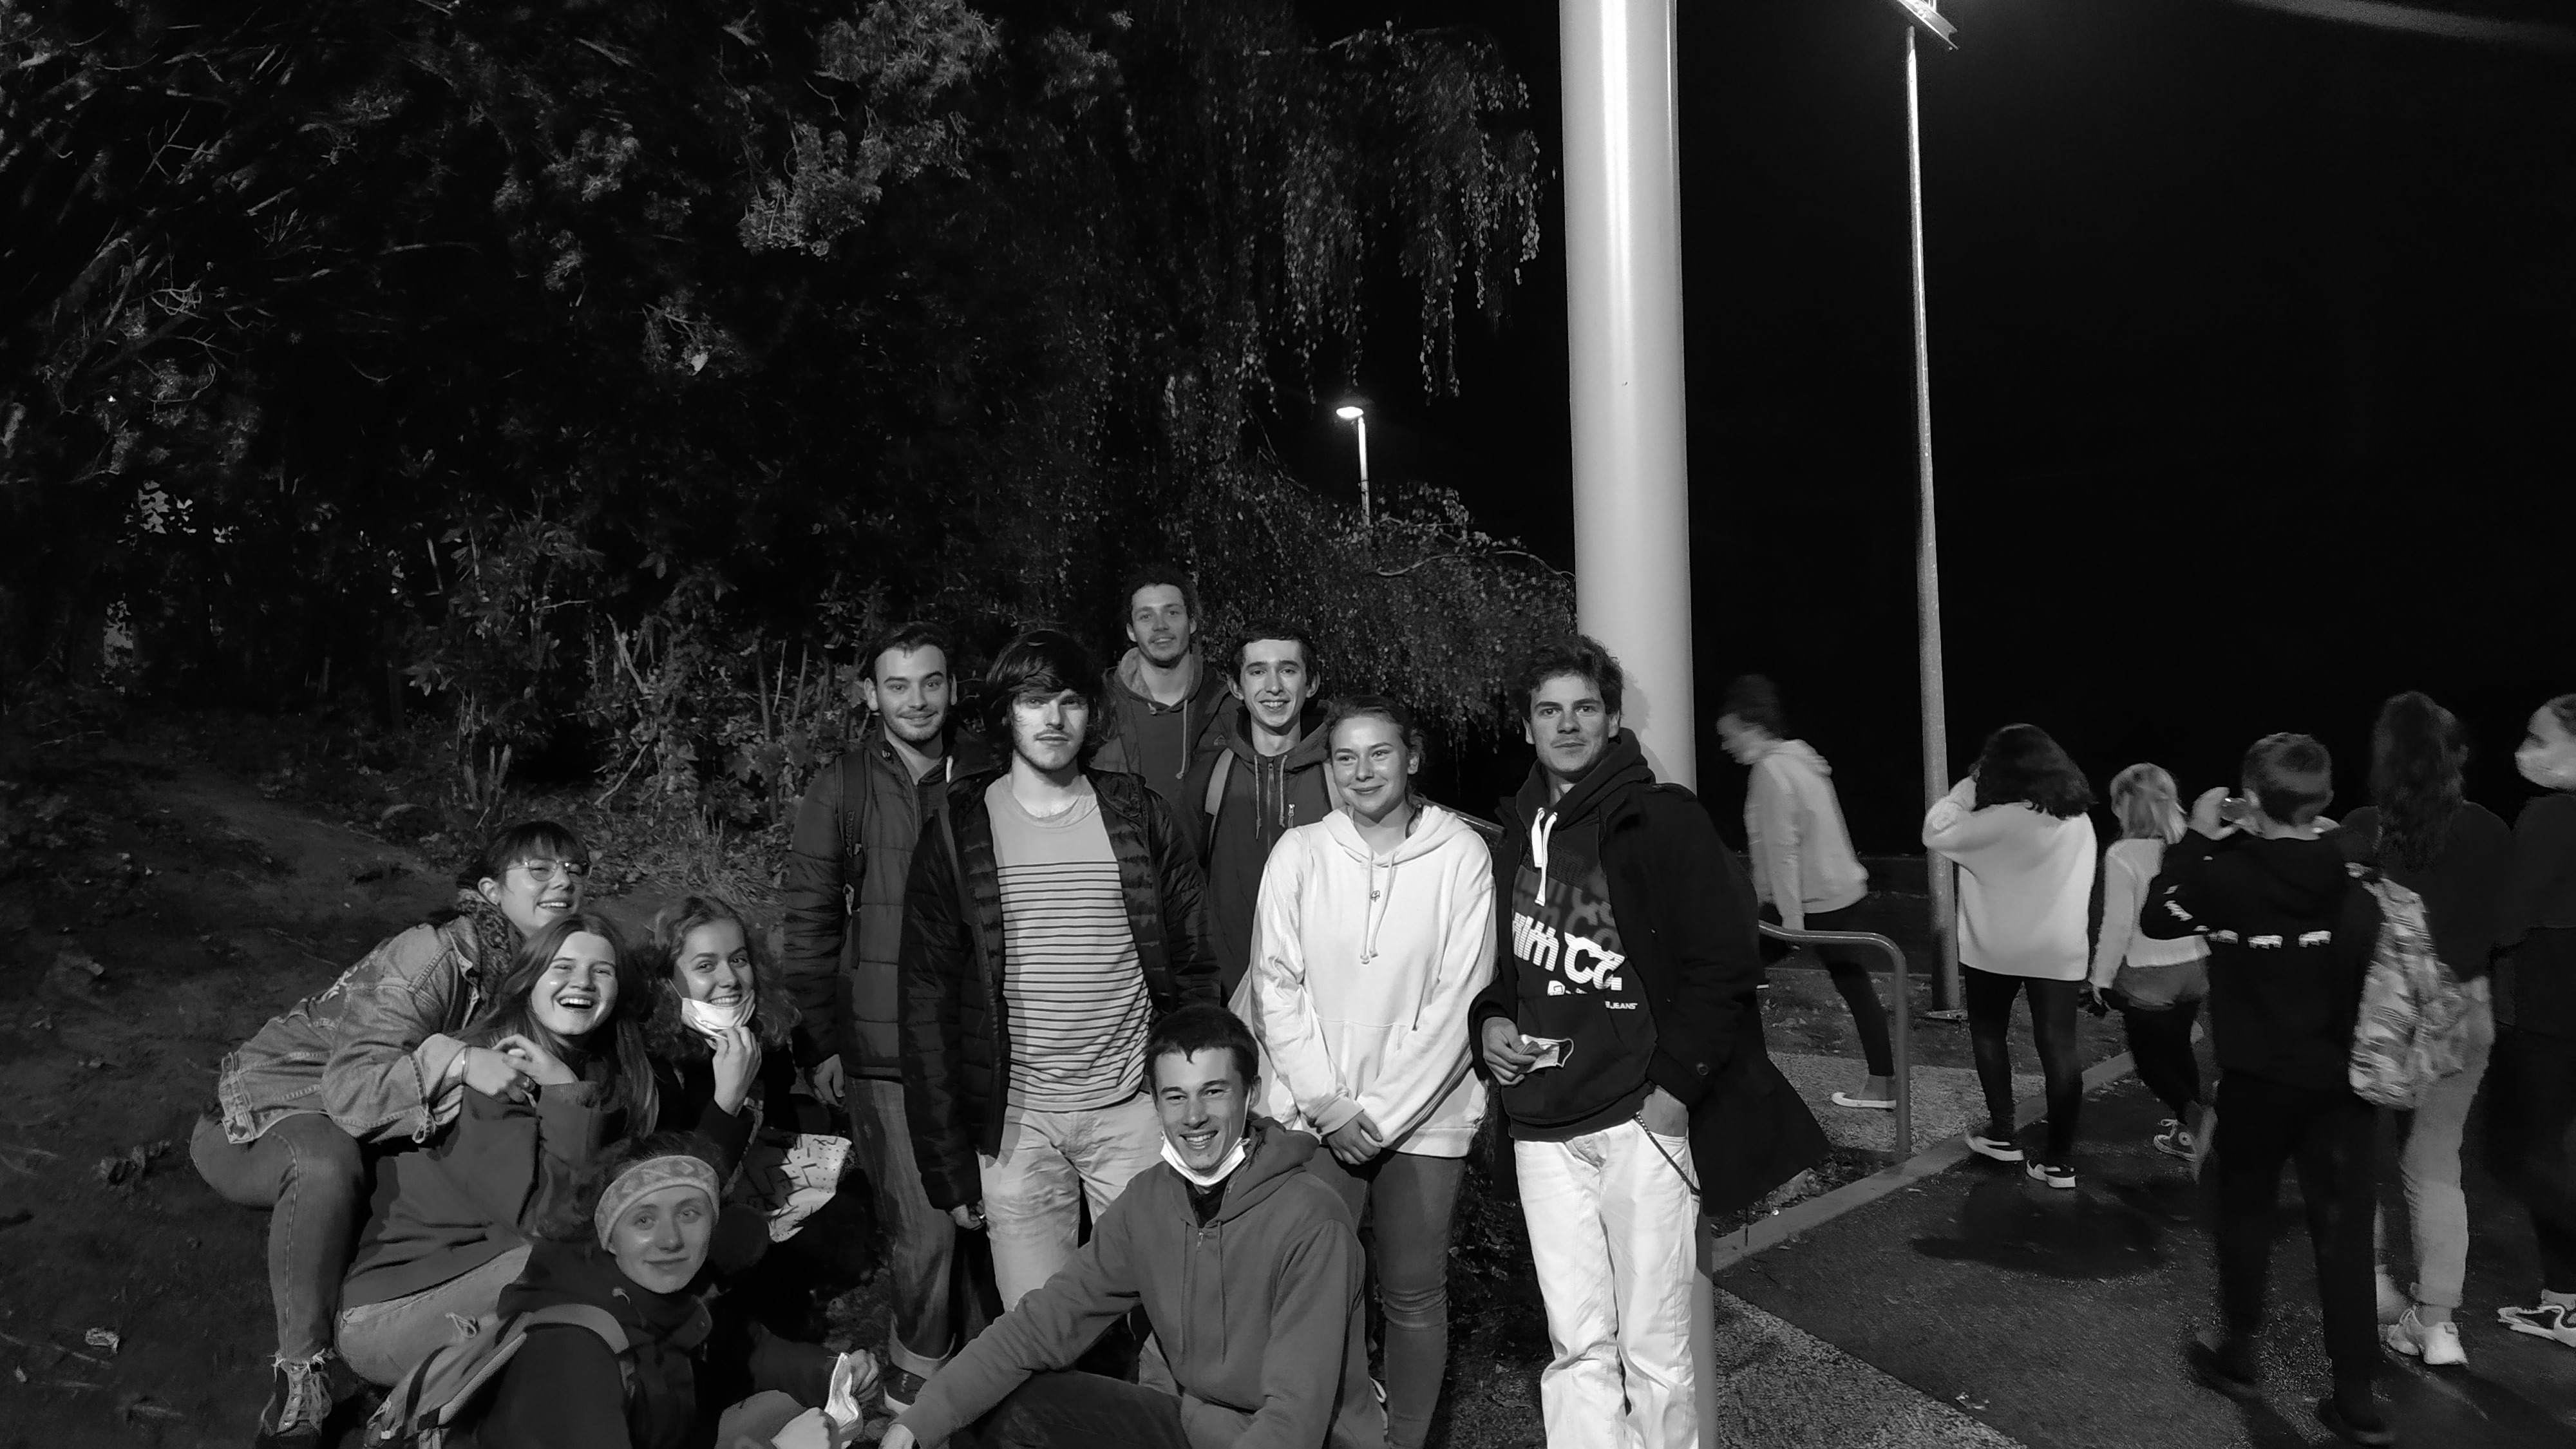
\includegraphics[width=1\linewidth, height=4cm]{patinoire_green}   
    \caption{Image des niveaux de gris du vert}
    \label{fig:patinoireGreen}
    \end{subfigure}
     \begin{subfigure}{0.6\textwidth}
    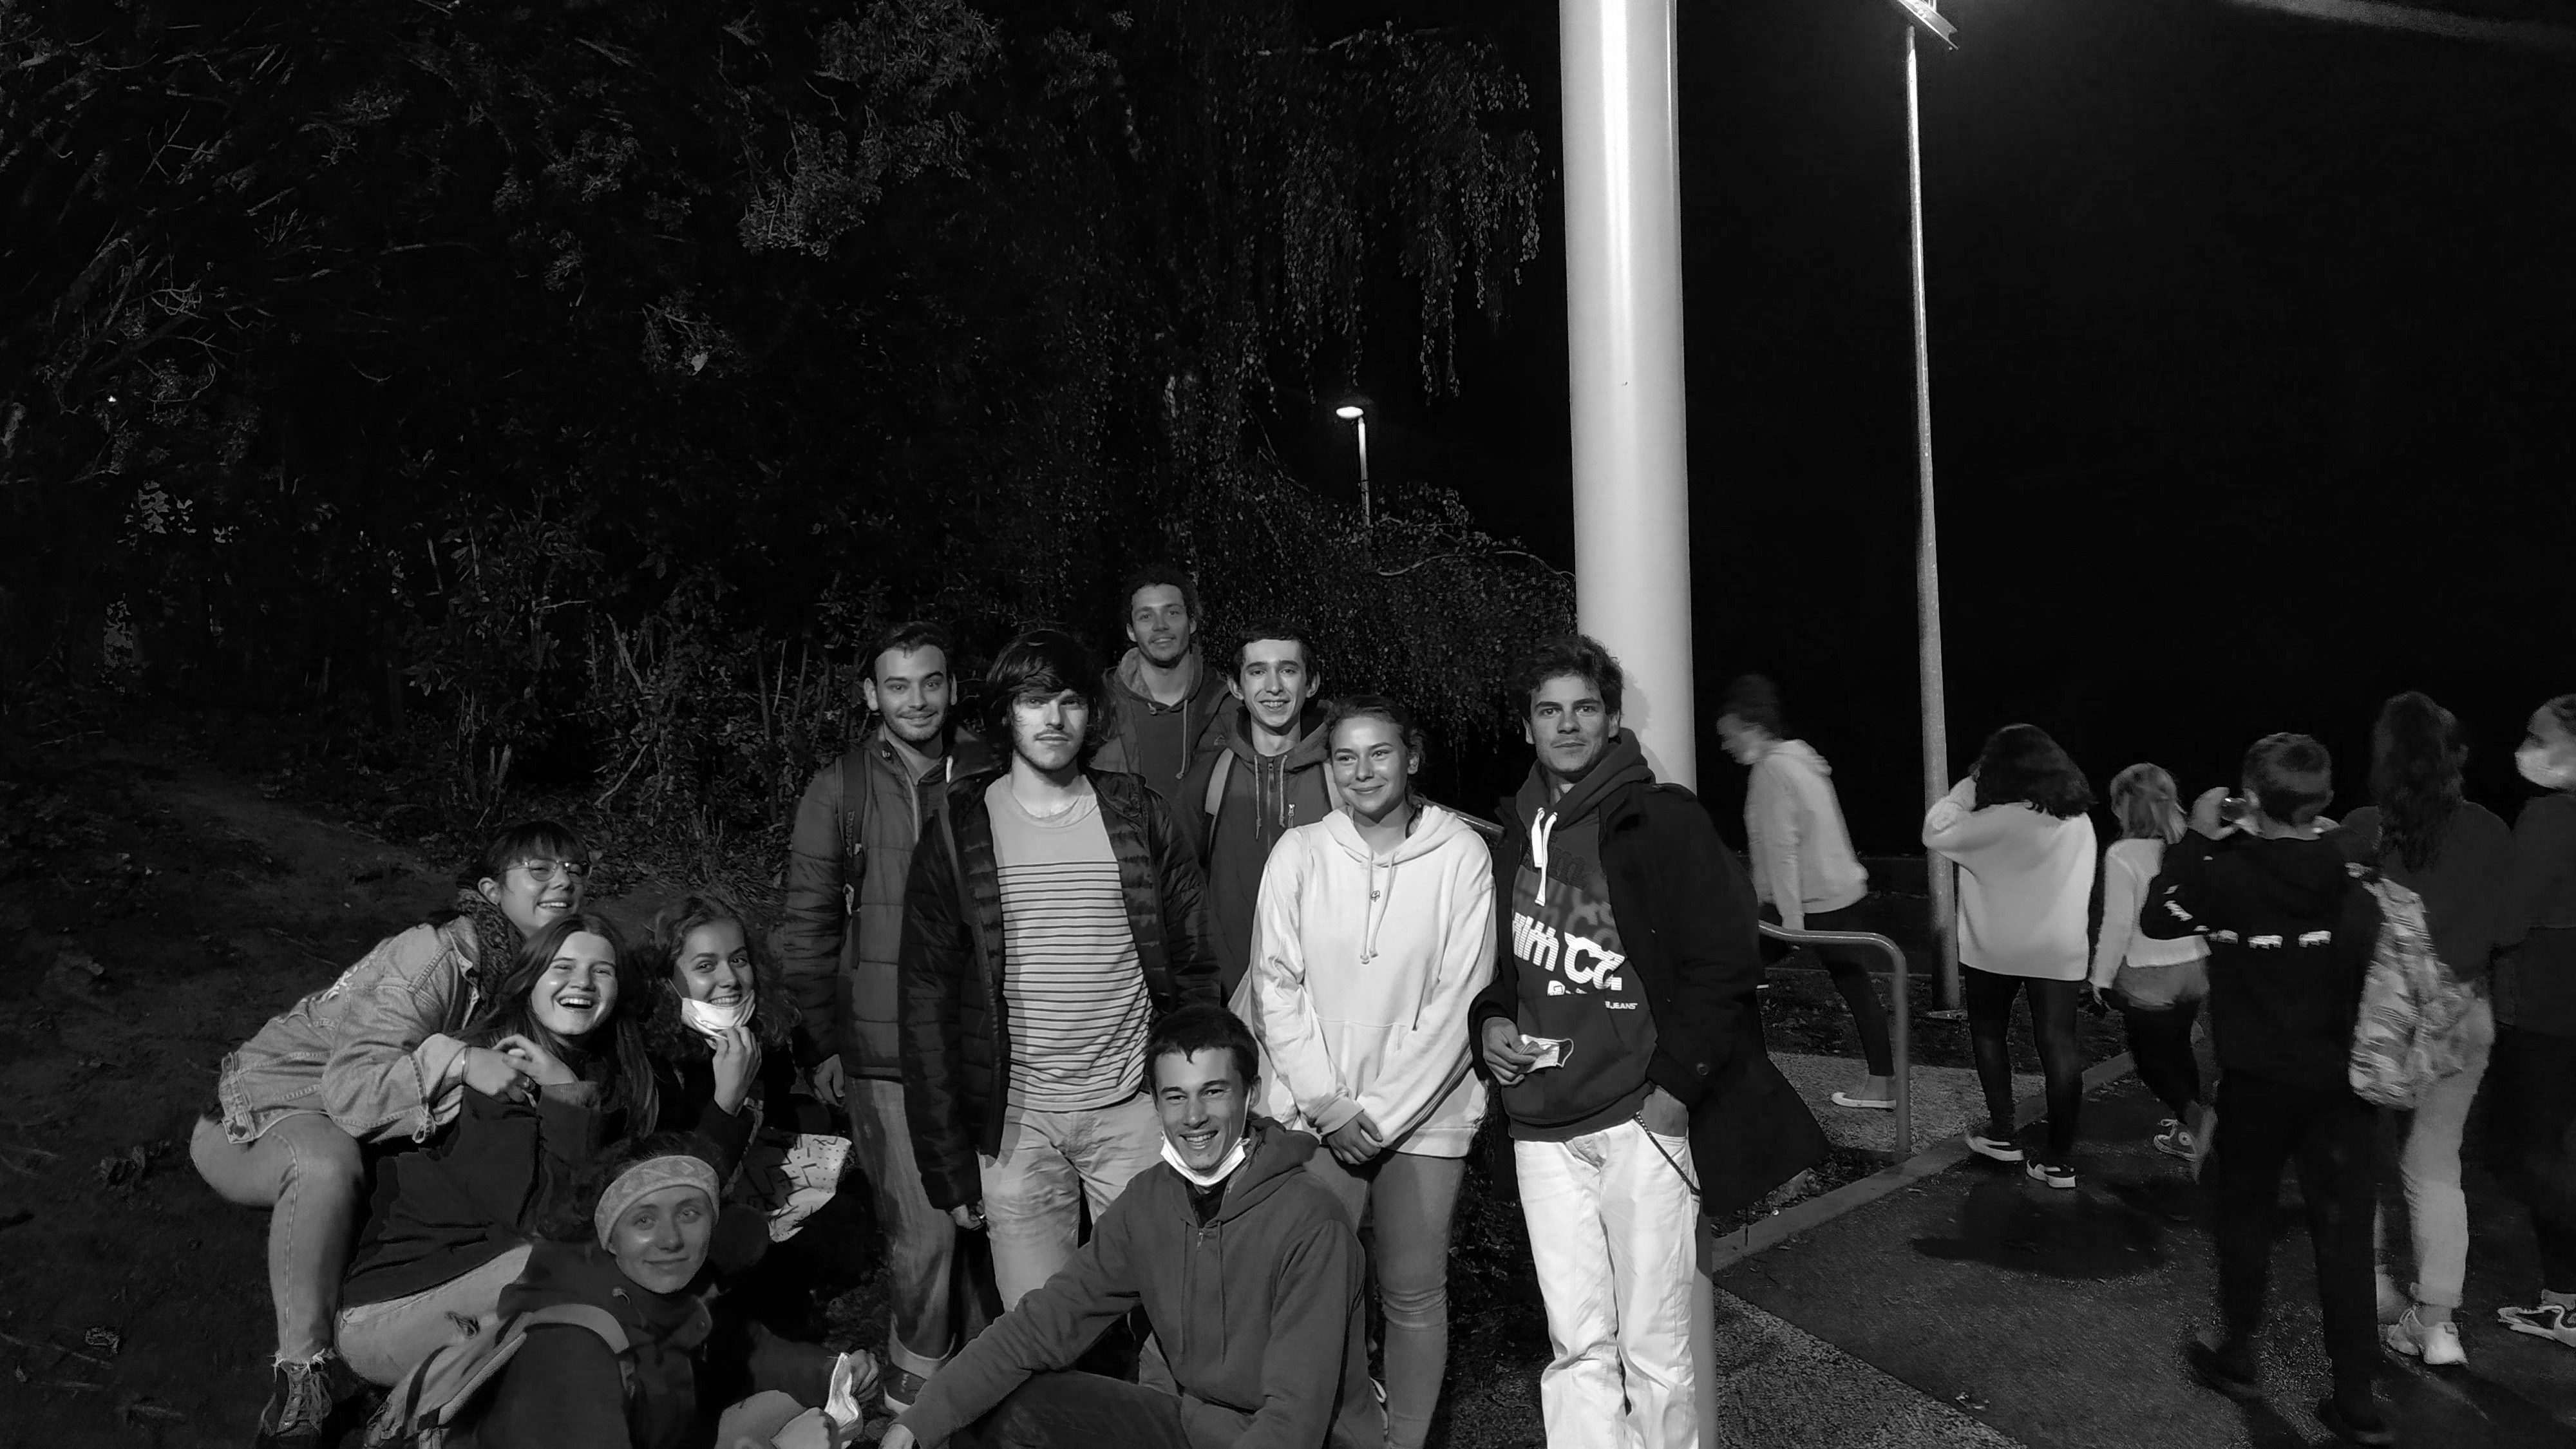
\includegraphics[width=1\linewidth, height=4cm]{patinoire_blue}   
    \caption{Image des niveaux de gris du bleu}
    \label{fig:patinoireBlue}
    \end{subfigure}
    \end{figure}
    \pagebreak
    \section{Itérateurs génériques non constants}
    Nous avons fait l'itérateur générique en lecture. Maintenant l'itérateur générique en lecture/écriture (i.e. non const).
     \begin{lstlisting}[language=Bash]
  $ ./save-all-channel dessin1.ppm dessin1_catho.ppm
  $ display dessin1_catho.ppm
  \end{lstlisting}
   \begin{figure}[h]
   \begin{subfigure}{0.6\textwidth}
    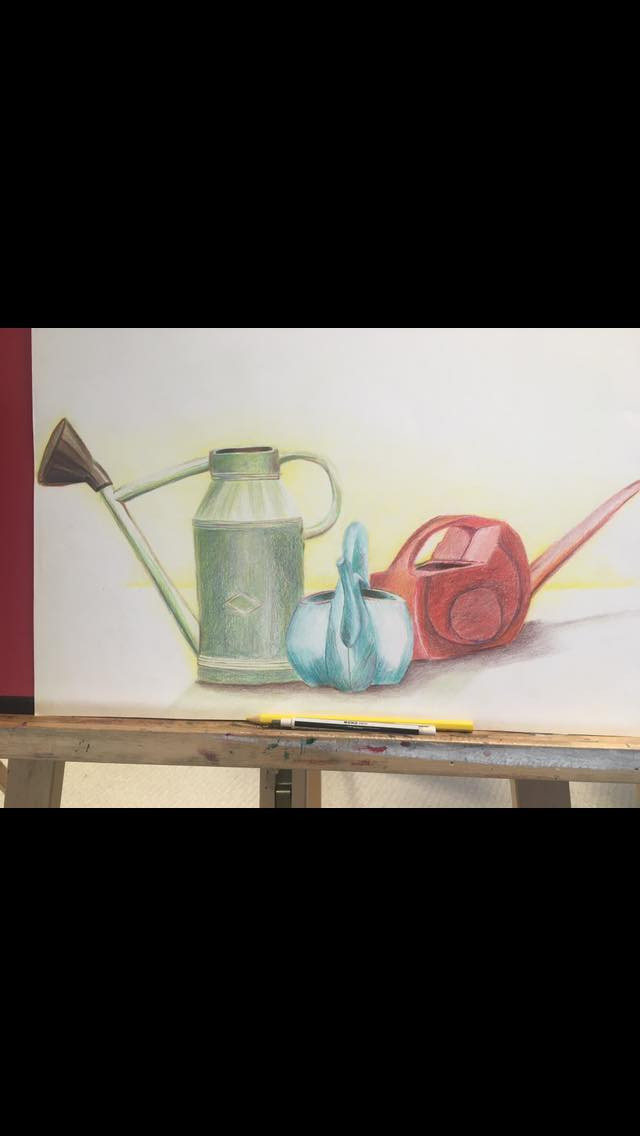
\includegraphics[width=1\linewidth, height=7cm]{dessin1}
    \caption{Image originale}
    \label{fig:dessin1Origin}
    \end{subfigure}
     \begin{subfigure}{0.6\textwidth}
    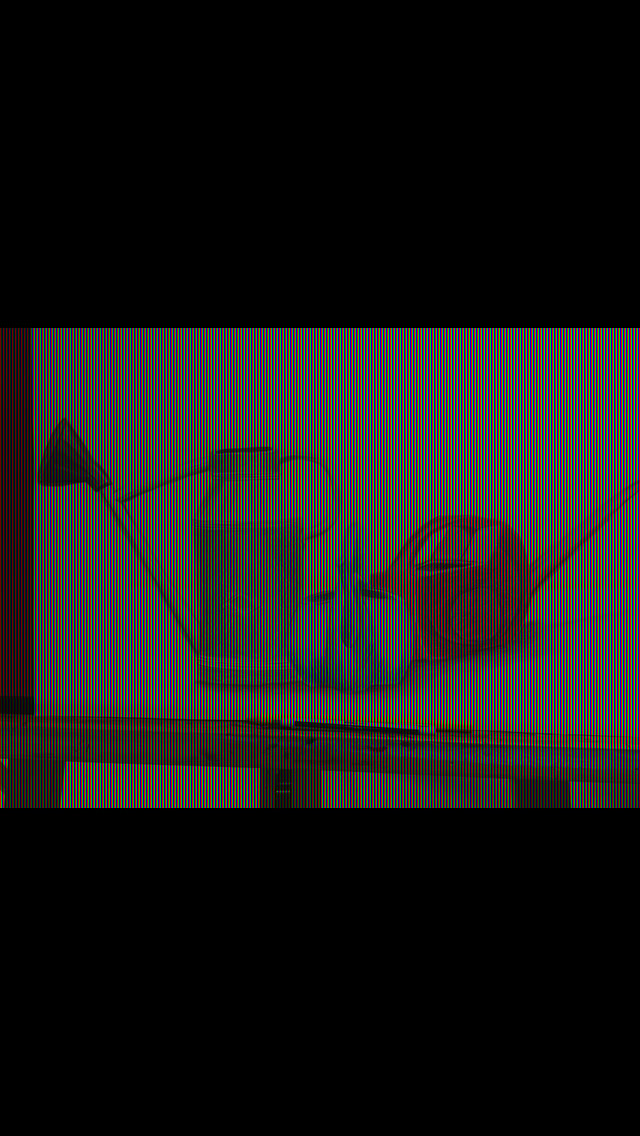
\includegraphics[width=1\linewidth, height=7cm]{dessin1_catho}   
    \caption{Image comme sur les écrans cathodiques}
    \label{fig:dessin1Catho}
    \end{subfigure}
    \end{figure}
    \pagebreak
    \section{Espace TSV (HSV) et histogramme d'une image couleur}
    Ici deux programmes, un pour faire des histogrammes sur les images en gris et l'autre pour faire des histogrammes sur les images couleurs.
    \begin{quote}
    D'abord celui en gris
    \end{quote}
    \begin{lstlisting}[language=Bash]
  $ ./histogrammeGrey lena.pgm lenaHisto.pgm     
  $ display lenaHisto.pgm
  \end{lstlisting}
  \begin{figure}[h]
   \begin{subfigure}{1\textwidth}
    \centering
    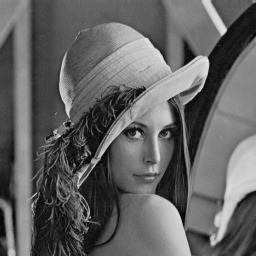
\includegraphics[width=0.6\linewidth, height=6cm]{lena}
    \caption{Image originale}
    \label{fig:lenaO}
    \end{subfigure}
     \begin{subfigure}{1\textwidth}
    \centering
    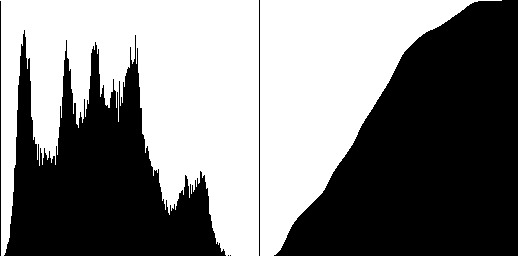
\includegraphics[width=1\linewidth, height=6cm]{lenaHisto}   
    \caption{Histogramme des niveaux de gris}
    \label{fig:lenaHisto}
    \end{subfigure}
    \end{figure}
    \pagebreak
    
    \begin{quote}
    Ensuite en couleur
    \end{quote}
    \begin{lstlisting}[language=Bash]
  $ ./histogrammeColor kowloon.ppm kowloonHisto.pgm     
  $ display kowloonHisto.pgm
  \end{lstlisting}
  \begin{figure}[h]
   \begin{subfigure}{1\textwidth}
    \centering
    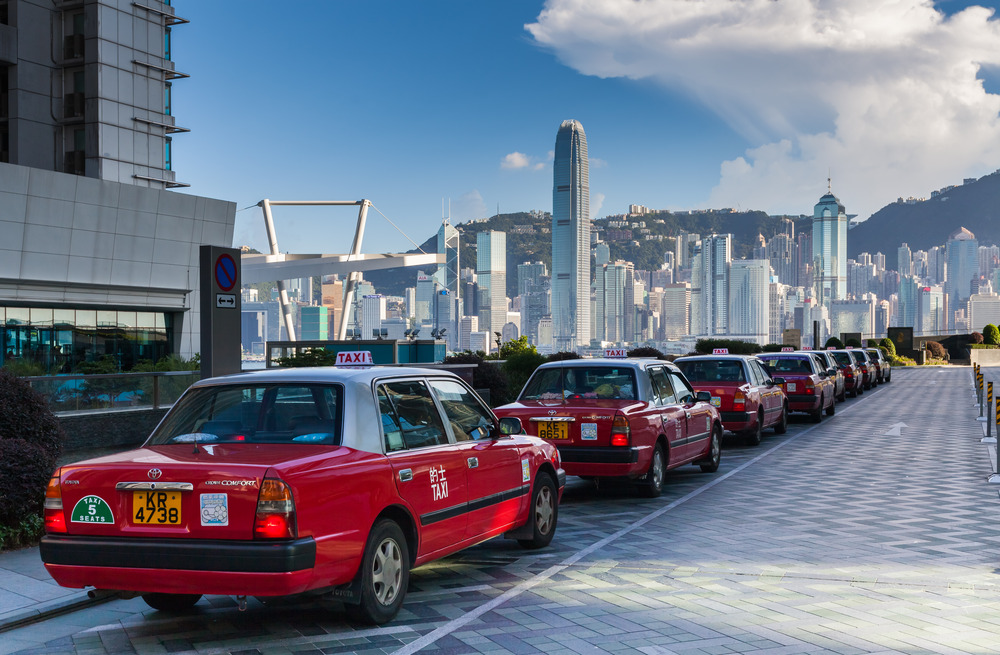
\includegraphics[width=0.8\linewidth, height=6cm]{kowloon}
    \caption{Image originale}
    \label{fig:kowloonO}
    \end{subfigure}
     \begin{subfigure}{1\textwidth}
    \centering
    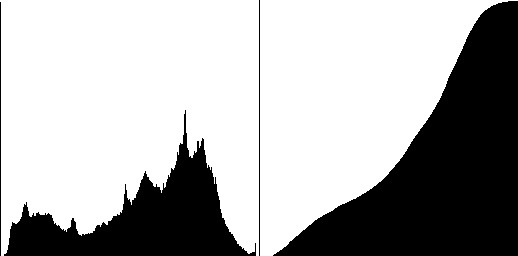
\includegraphics[width=1\linewidth, height=6cm]{kowloonHisto}   
    \caption{Histogramme des niveaux de couleur}
    \label{fig:kowloonHisto}
    \end{subfigure}
    \end{figure}

    \pagebreak
    \section{Egalisation d'image couleur}
    Dès que l'on a un histogramme cumulé d'une image, il est maintenant facile d'égaliser l'image pour la rendre bien balancé. On utilisera cette fonction d'égalisation mais sur les valeurs des couleurs, via nos itérateurs génériques avec accesseur ColorValueAccessor. 
    \begin{lstlisting}[language=Bash]
      $ ./egaliseur kowloon.ppm    
      $ display kowloon_histoEq.pgm
      & display kowloon_egalise.pgm
    \end{lstlisting}

    \begin{figure}[h]
      \begin{subfigure}{0.5\textwidth}
        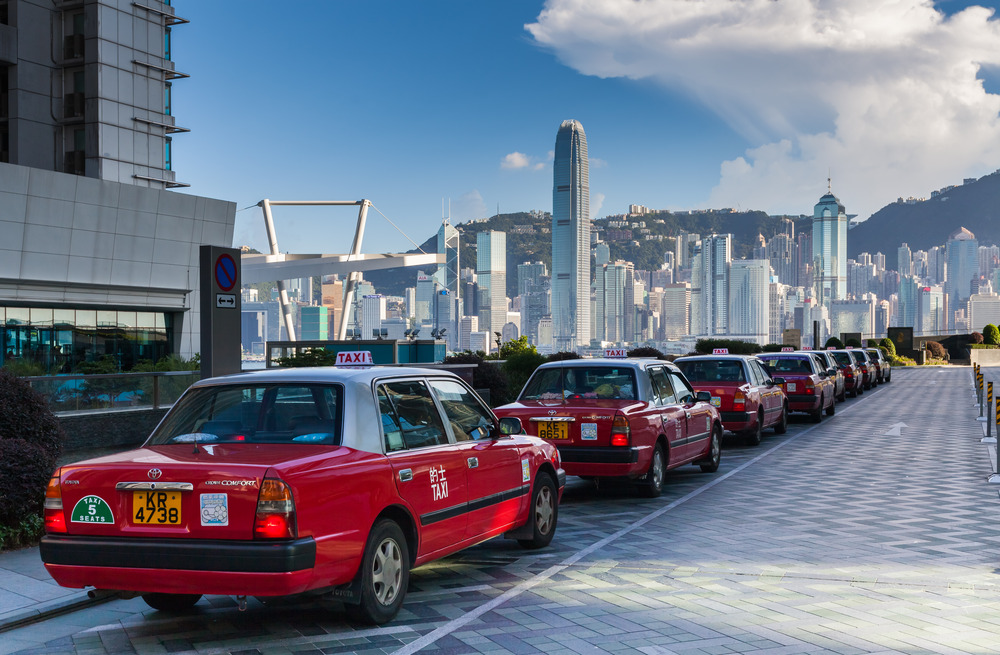
\includegraphics[width=1\linewidth, height=4cm]{kowloon}
        \caption{Image originale}
        \label{fig:kowloonO}
      \end{subfigure}
      \begin{subfigure}{0.5\textwidth}
        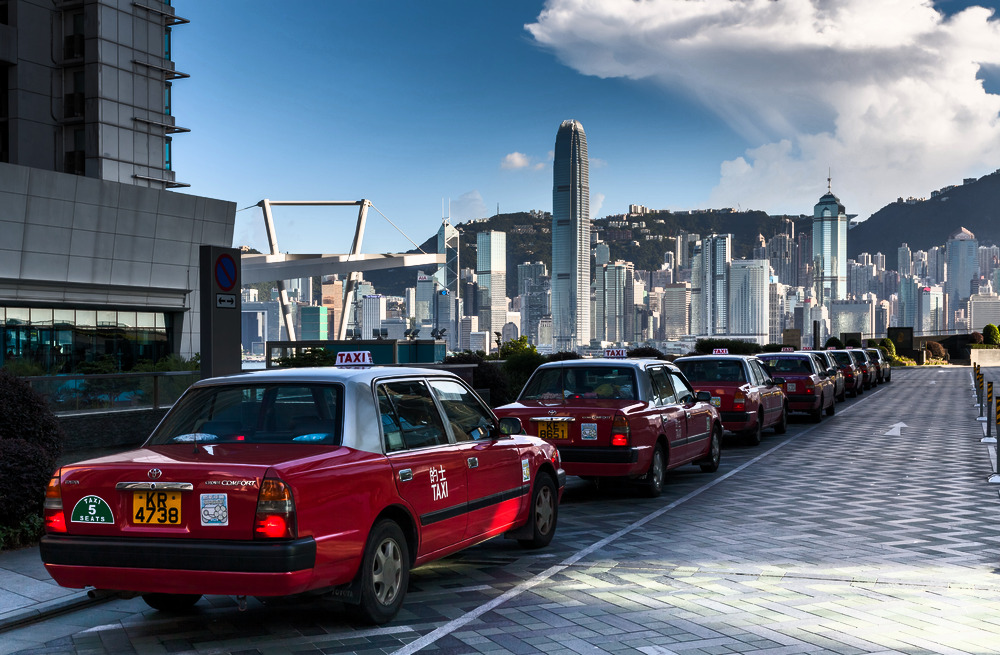
\includegraphics[width=1\linewidth, height=4cm]{kowloon_egalise.jpeg}
        \caption{Image égalisée}
        \label{fig:kowloonO}
      \end{subfigure}
      \begin{subfigure}{1\textwidth}
        \centering
        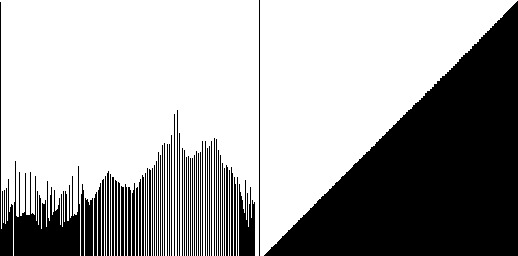
\includegraphics[width=1\linewidth, height=6cm]{kowloon_histoEq.jpeg}   
        \caption{Histogramme des niveaux de couleur égalisée}
        \label{fig:kowloonHisto}
      \end{subfigure}
    \end{figure}

    \pagebreak
    \section{Un peu d'imagination}
    \subsection{Inversion des couleurs}
    Petit programme qui permet d'inverser les valeurs des couleurs d'une image.
\end{document}
